\documentclass{article}

\newcommand{\ep}{\rule{.06in}{.1in}}
\textheight 9.5in

\usepackage{amssymb}
\usepackage{amsmath}
\usepackage{amsthm}
\usepackage{graphicx, subcaption, booktabs}
\graphicspath{{/Users/andrewwork/thesis/jump-velocity/plots/}}

\usepackage{tikz, pgfplots, pgfplotstable, chemfig}

% \usepgfplotslibrary{colorbrewer, statistics}
% \pgfplotsset{
%   exact axis/.style={grid=major, minor tick num=4, xlabel=$v^*$,
%     legend entries={PDF, CDF},},
%   every axis plot post/.append style={thick},
%   table/search
%   path={/Users/andrewwork/thesis/jump-velocity/dat-files},
%   colormap/YlGnBu,
%   cycle list/Set1-5,
%   legend style={legend cell align=left,},
% }

% \usepgfplotslibrary{external}
% \tikzexternalize

\renewcommand{\arraystretch}{1.2}
\pagestyle{empty} 
\oddsidemargin -0.25in
\evensidemargin -0.25in 
\topmargin -0.75in 
\parindent 0pt
\parskip 12pt
\textwidth 7in
%\font\cj=msbm10 at 12pt

\newcommand{\tn}{\textnormal}
\newcommand{\stiff}{\frac{k_f}{\gamma}}
\newcommand{\dd}{d}
\newcommand{\Der}[2]{\frac{\dd #1}{\dd #2}}
\newcommand{\Pder}[2]{\frac{\partial #1}{\partial #2}}
\newcommand{\Integral}[4]{\int_{#3}^{#4} {#1} \dd #2}
\DeclareMathOperator{\Exp}{Exp}

% Text width is 7 inches

\def\R{\mathbb{R}}
\def\N{\mathbb{N}}
\def\C{\mathbb{C}}
\def\Z{\mathbb{Z}}
\def\Q{\mathbb{Q}}
\def\H{\mathbb{H}}
\def\B{\mathcal{B}} 
%\topmargin -.5in 

\setcounter{secnumdepth}{2}
\begin{document}
\pagestyle{plain}

\begin{center}
  {\Large Meeting Notes (\today)}
\end{center}

{\Large \textbf{Integrating Platelet Motion}}

\textbf{Equations of motion for the platelet}
\begin{itemize}
\item The translational and angular velocities can be found using
  force (and torque) balance on the platelet:
  \[
    0 = F^\tn{drag} + F^\infty + F^\tn{other}
  \]
  \begin{itemize}
  \item $F^\tn{drag}$ is the drag force on a platelet moving with
    velocity $U$ through a stationary fluid, and is the product of the
    resistance matrix $R$ and the (translational and angular) velocities
    $U$: $F^\tn{drag} = RU$
  \item $F^\infty$ is the drag force on a platelet that is stationary in
    the background flow. For us, this would be a shear flow with shear
    rate $\gamma$: $\mathbf{v}^\infty = \gamma x \mathbf{e}_z$
  \item $F^\tn{other}$ are any other forces acting on the platelet;
    particularly bond forces and other chemical forces
  \end{itemize}
\item The platelet velocities can be found by inverting the resistance
  matrix: $U = -R^{-1}\left(F^\infty + F^\tn{other}\right)$
\item Then define the 3 translational velocities and 3 angular
  velocities as $v_x$, $v_y$, $v_z$ and $\omega_x, \omega_y, \omega_z$.
\item Let $x$, $y$, and $z$ be the position of the platelet center of
  mass, and $\theta$ and $\phi$ define the platelet's orientation (see
  Figure \ref{fig:sketches} below). All of these quantities are
  functions of time, $t$.
\item The platelet's position over time satisfies
  $\dfrac{dx}{dt} = v_x$ (and similar for $y$ and $z$)
\item The platelet's orientation satisfies
  \begin{align*}
    \frac{d\theta}{dt} &= \omega_x - \omega_y \cos\theta \cot\phi -
                         \omega_z \sin\theta \cot\phi \quad \tn{and} \\
    \frac{d\phi}{dt} &= \omega_z \cos\theta - \omega_y \sin\theta
  \end{align*}
\item To start with, I'm using Forward Euler to integrate the platelet
  motion
\item Potential problem? $\dfrac{d\theta}{dt}$ is undefined at
  $\phi = 0$ and $\phi = \pi$. If $\phi$ is close to these values, I'd
  expect Forward Euler to be much less accurate (and could stability
  be an issue?).
\end{itemize}

\begin{figure}
  \centering
  \begin{subfigure}{0.59\textwidth}
    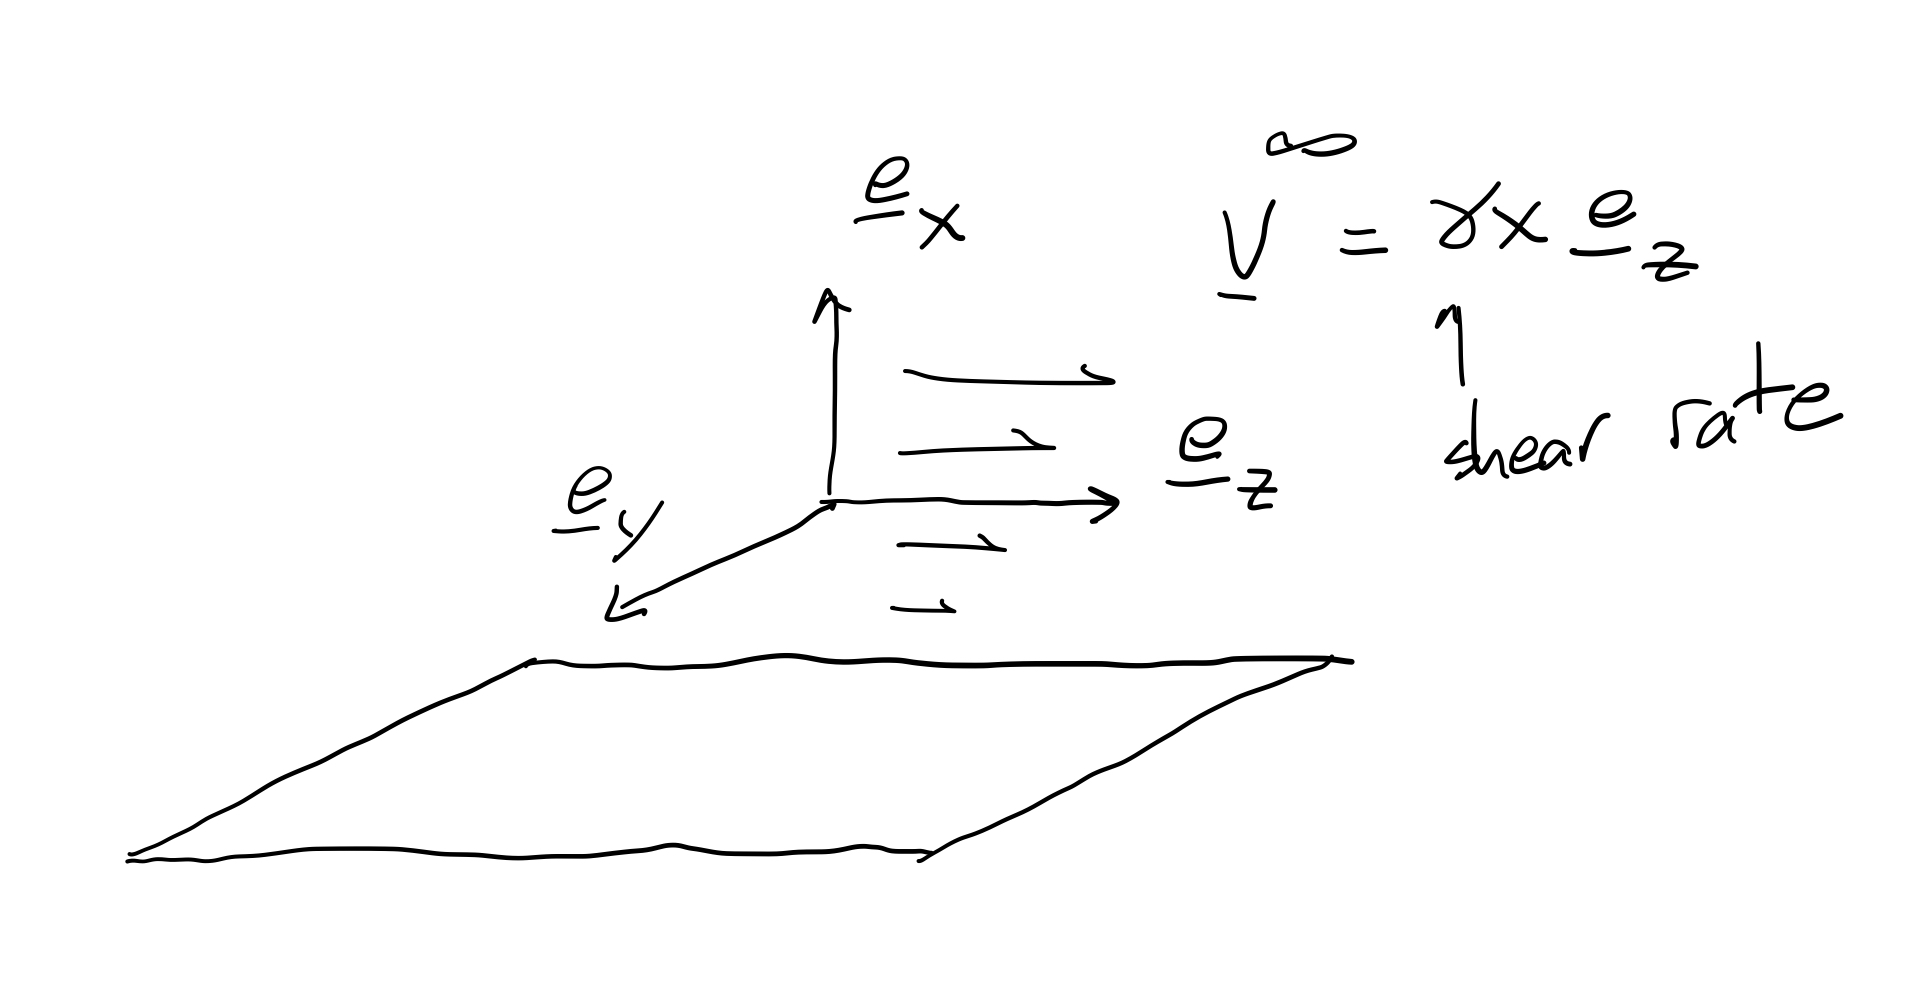
\includegraphics[width=\textwidth]{axes}
  \end{subfigure}
  \hfill
  \begin{subfigure}{0.39\textwidth}
    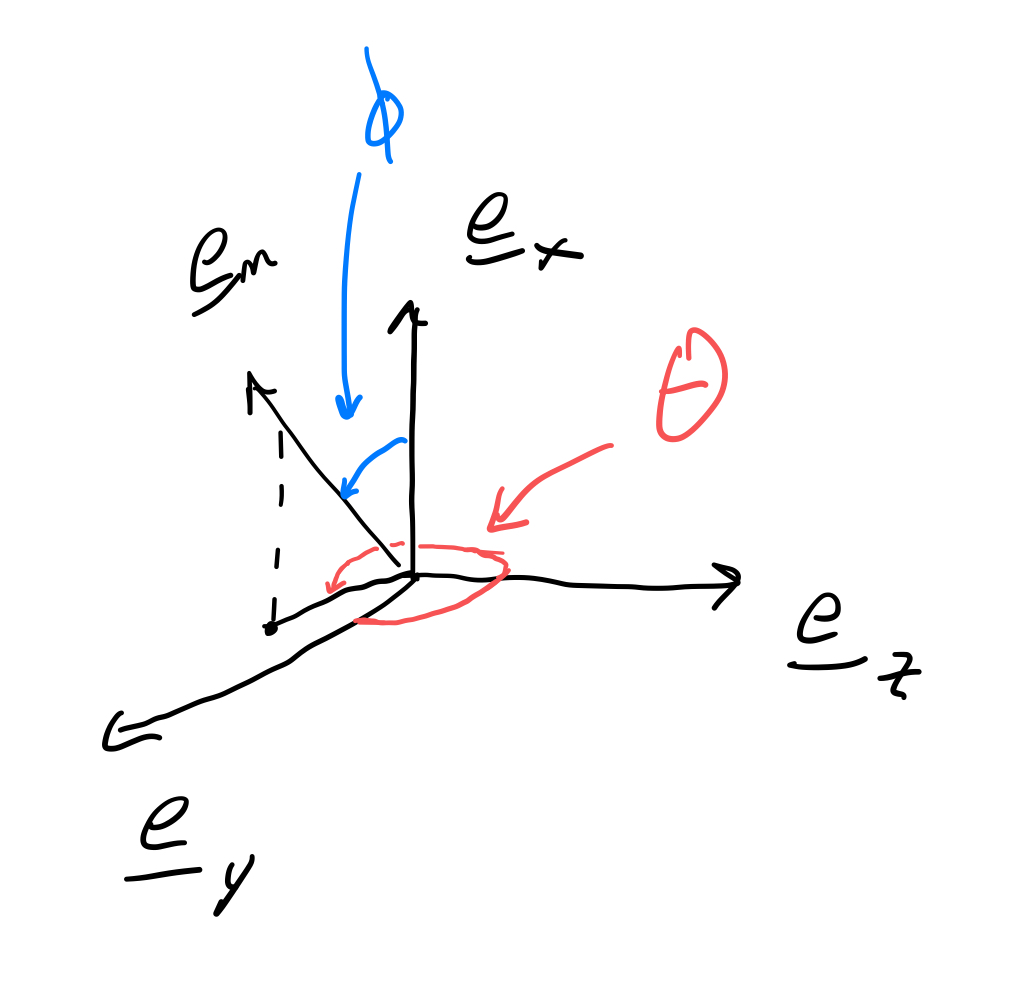
\includegraphics[width=\textwidth]{orientation}
  \end{subfigure}
  \\
  \begin{subfigure}{0.49\textwidth}
    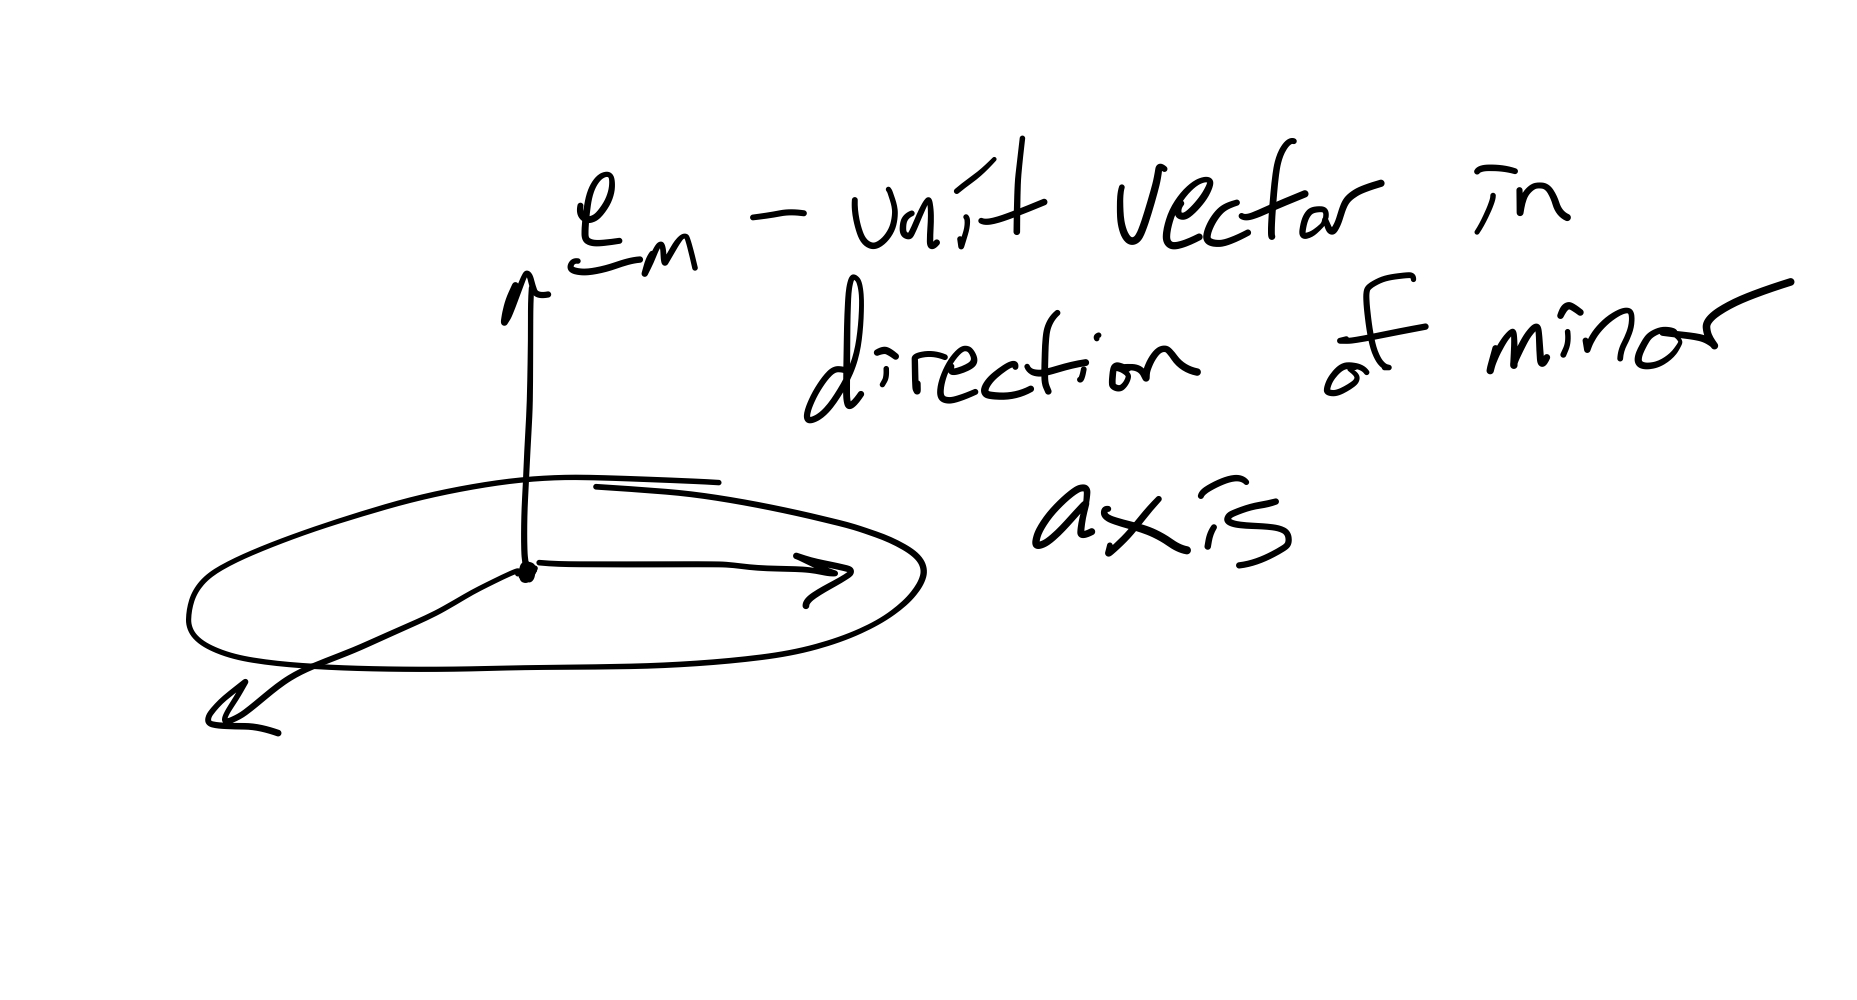
\includegraphics[width=\textwidth]{reference}
  \end{subfigure}
  \caption{Sketch of the axes and orientation angles of the ellipsoid}
  \label{fig:sketches}
\end{figure}

\textbf{Test Case: Sphere in an unbounded shear flow}
\begin{itemize}
\item The first test case I tried was a sphere in an unbounded shear
  flow. The velocity of the sphere in this case is $v_x = v_y = v_z =
  0$ (assuming $x = 0$), and the angular velocities are $\omega_x =
  \omega_z = 0$ and $\omega_y = \gamma/2$.
\item Therefore with $\gamma = 1$, $\dfrac{d\theta}{dt} = \dfrac{1}{2}
  \dfrac{\cos\theta}{\tan\phi}$ and $\dfrac{d\phi}{dt} = \dfrac{1}{2}
  \sin\theta$.
\item I integrated this system of DEs to get ``exact'' values of
  $\theta$ and $\phi$ as a function of time, and compared with the
  routine described above using regularized Stokeslets (results in
  Figure \ref{fig:com_plot})
\item Note: in this test case, the regularized Stokeslets routine
  gives translational and angular velocities that are exact within
  machine precision (I don't really know why, perhaps because of
  symmetry we get mirrored errors that cancel each other out
  somehow). Therefore the error that is shown in Figure
  \ref{fig:com_plot} is only due to the Forward Euler integration.
\end{itemize}

\begin{figure}
  \centering
  \begin{subfigure}{0.49\textwidth}
    \includegraphics[width=\textwidth]{com_plot}    
  \end{subfigure}
  \hfill
  \begin{subfigure}{0.49\textwidth}
    \includegraphics[width=\textwidth]{orient_plot}
  \end{subfigure}
  \caption{Plots of the platelet position and orientation in an
    unbounded shear flow. Orientation is initialized at $\theta = 0$
    and $\phi = \pi/8$.}
  \label{fig:com_plot}
\end{figure}

\newpage

\textbf{Test Case: Sphere in a shear flow, adjacent to a wall}
\begin{itemize}
\item For the second test case, place a sphere in a shear flow near a
  plane wall.
\item Goldman, Cox, and Brenner \cite{Goldman1967b} assemble results
  for the free motion of a sphere in this case. The only nonzero
  components of the velocity are $v_z$ and $\omega_y$.
\item With the center of mass at $x = h = 1.5431$, $y = z = 0$, the
  translational velocity is $v_z = 0.92185 h$ and the rotational
  velocity is $\omega_y = 0.92368 / 2$
\item The regularized Stokeslets code for this test case is currently
  failing. The angular velocities are correct, but the translational
  velocity produced by the regularized Stokeslets are roughly half
  what they should be (Figure \ref{fig:com_plot2})
\item The source of this error seems to be in computing the upper
  right block of the resistance matrix:
  $R =
  \begin{pmatrix}
    \mathcal{T} & \mathcal{P} \\
    \mathcal{P}^T & \mathcal{R}
  \end{pmatrix}$

\end{itemize}

\begin{figure}
  \centering
  \begin{subfigure}{0.49\textwidth}
    \includegraphics[width=\textwidth]{com_plot2}
  \end{subfigure}
  \hfill
  \begin{subfigure}{0.49\textwidth}
    \includegraphics[width=\textwidth]{orient_plot2}
  \end{subfigure}
  \caption{Plots of the platelet position and orientation in a shear
    flow near a wall. Same as the previous example, orientation is
    initialized at $\theta = 0$ and $\phi = \pi/8$}
  \label{fig:com_plot2}
\end{figure}

\bibliographystyle{plain}
\bibliography{/Users/andrewwork/Documents/grad-school/thesis/library}

\end{document}




